% file: stack-sites/qtree-node-newcommand.tex

\documentclass[tikz]{standalone}

\usepackage{tikz-qtree}

\newcommand{\lnode}[3]{\node [label = {#1} : {$#2$}] {#3};}

\begin{document}
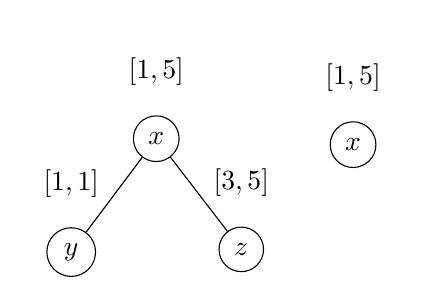
\begin{tikzpicture}[level distance = 40pt, sibling distance = 30pt,
  edge from parent/.style= {
  	draw, edge from parent path={(\tikzparentnode) -- (\tikzchildnode)}}]
  \tikzset{every node/.style = {draw, circle}}

  \lnode{above}{[1,5]}{$x$} 

  \begin{scope}[xshift = -2.5cm]
    \Tree [.\node[label = above : {$[1,5]$}]{$x$}; 
	    [.\node[label = above : {$[1,1]$}] {$y$}; ] 
	    [.\node[label = above : {$[3,5]$}] {$z$}; ]
	  ]
  \end{scope}

  % \lnode does not work in qtree
  % \begin{scope}[xshift = 2.5cm]
  %   \Tree [.\lnode{above}{[1,5]}{$x$}
  %           [.\lnode{above}{[1,1]}{$y$} ]
  %           [.\lnode{above}{[3,5]}{$z$} ]
  %         ]
  % \end{scope}
\end{tikzpicture}
\end{document}
